%
% File emnlp2018.tex
%
%% Based on the style files for EMNLP 2018, which were
%% Based on the style files for ACL 2018, which were
%% Based on the style files for ACL-2015, with some improvements
%%  taken from the NAACL-2016 style
%% Based on the style files for ACL-2014, which were, in turn,
%% based on ACL-2013, ACL-2012, ACL-2011, ACL-2010, ACL-IJCNLP-2009,
%% EACL-2009, IJCNLP-2008...
%% Based on the style files for EACL 2006 by
%%e.agirre@ehu.es or Sergi.Balari@uab.es
%% and that of ACL 08 by Joakim Nivre and Noah Smith

\documentclass[11pt,a4paper]{article}
\usepackage[hyperref]{emnlp2018}
\usepackage{times}
\usepackage{latexsym}
\usepackage{url}
\usepackage{amsmath}
\usepackage{algorithm}
\usepackage{algorithmic}
%%% YOUR PACKAGES BELOW THIS LINE %%%
\usepackage[small,bf]{caption} % added MLF 20171211
\usepackage{multicol}
\usepackage{adjustbox}
\usepackage{graphicx}
\usepackage{array,multirow}
%\aclfinalcopy % Uncomment this line for the final submission

\setlength\titlebox{5cm}
% You can expand the titlebox if you need extra space
% to show all the authors. Please do not make the titlebox
% smaller than 5cm (the original size); we will check this
% in the camera-ready version and ask you to change it back.

\newcommand\BibTeX{B{\sc ib}\TeX}
\newcommand\confname{EMNLP 2018}
\newcommand\conforg{SIGDAT}

\title{Crosslingual Sentence Embeddings for Neural Machine Translation}
%\title{A Recurrent Network for Parallel Corpora Divergence Analysis}

\author{%Minh Pham, \ Fran\c cois Yvon\\
  First author\\
  Affiliation / Address line 1\\
  Affiliation / Address line 2\\
  Affiliation / Address line 3\\
  {\tt email@domain}  
  \And
  %Josep Crego, \ Jean Senellart\\
  Second author\\
  Affiliation / Address line 1\\
  Affiliation / Address line 2\\
  Affiliation / Address line 3\\
  {\tt email@domain}}

\date{}

\begin{document}
\maketitle
\begin{abstract}

%http://www.airccj.org/CSCP/vol4/csit42503.pdf

Corpus-based approaches to machine translation rely on the availability and quality of parallel corpora.
In the case of neural machine translation, a large neural network is trained to maximise the translation performance on a given parallel corpus. 
%This paper describes an unsupervised method for building cross lingual sentence embeddings, which can then be used to compute semantic similarity between sentences in different languages.
This paper describes an unsupervised method for building cross-lingual
sentence embeddings that optimise word alignments. Such embeddings can then be used to compute semantic similarity between sentences in different languages.
We report competitive performance on two different tasks. 
Sentence embeddings are first used to detect translation divergences
in parallel sentence pairs, therby helping to filter out noisy pairs.
Then, sentence embeddings help to discover parallel sentences in comparable corpora.
We evaluate our model on multiple language pairs and data resources.
This model can be used on any parallel corpus without any manual annotation.

%According to the process followed to compile a parallel corpus, it may contain multiple parallel sentences that are often not as parallel as one might assume. Examples are easily found when corpora is created from non-parallel texts or included by noisy document/sentence alignment tools.
%This paper describes an unsupervised method for detecting translation divergencies in parallel sentence pairs. We use a deep neural network to predict word alignment scores in parallel sentences. Misaligned words are then identified allowing divergent parallel sentences to be filtered out and in some cases making sentences parallel by removing such words. 
%We evaluate the presented method on a machine translation task. Results show that a neural MT system trained on the filtered/corrected sentences outperforms the neural MT system trained on the original sentence pairs. This method can be used on any parallel corpus without any manual annotation.

\end{abstract}

\section{Introduction}

Parallel sentence pairs are the only necessary resource to build Machine Translation (MT) systems.
In the case of neural MT, a large neural network is trained through maximising translation performance on a given parallel corpus. 
Therefore, the quality of an MT engine is heavily dependent upon the
amount and quality of the training parallel sentences.\footnote{Note
  that  recent work on neural MT
  \cite{lample2018word,artetxe2018iclr} completely dispenses with the
  need of parallel data, using unsupervised methods to obtain performance
  improvements over word-by-word statistical MT systems. However, these systems
  still lag far behind systems trained in a supervised fashion, as
  considered in this work.} 

Unfortunately, parallel texts are scarce resources. 
There are relatively few language pairs for which parallel corpora of
reasonable sizes are available, and even for those pairs, the corpora
are only representative of a small number of domains or genres. 
To mitigate the lack of parallel data, several approaches have been developed in the last years.
They range from methods using non-parallel, or comparable data ~\cite{Zhao:2002:APS:844380.844785,W04-3208,J05-4003,W17-2509,P17-3003,P18-2037} to techniques that produce synthetic parallel data from monolingual corpora ~\cite{P16-1009,W17-4714} using in all cases automated alignment/translation engines that are prone to introducing noise in the resulting parallel sentences. 
Mismatches in parallel sentences extracted from translated texts are also reported ~\cite{tiedemann2011bitext,XU16.310}. 
This problem is mostly ignored in MT, where parallel sentences are considered to convey the exact same meaning, but seems particularly important for neural MT engines, as noted in~\citet{chen2016adaptation}.

Table~\ref{tab:examples} gives some examples of English-French
parallel sentences that are not completely semantically equivalent, 
extracted from the OpenSubtitles corpus ~\cite{LisonTiedemann2016}. 
Divergences are outlined using bold letters. 

\begin{table}[ht]
%\begin{adjustbox}{width=0.48\textwidth}
\small
\center
\begin{tabular}{ c|l }
  %\hline
  \hline  
  \texttt{en} & \it{What do you feel}\bf{, Spock}\it{?} \\
  \texttt{fr} & \it{Que ressentez-vous?} \\
  \texttt{gl} & {\small \it{What do you feel?}} \\
  \hline
  \texttt{en} & \it{How much do you get paid?} \\
  \texttt{fr} & \it{T'es pay\'e combien} \bf{de l'heure}\it{?} \\
  \texttt{gl} & {\small \it{How much do you get paid per hour?}} \\
  \hline  
  \texttt{en} &  \bf{That seems a lot.} \\
  \texttt{fr} & \bf{40 livres?} \\
  \texttt{gl} & {\small \it{40 pounds?}} \\
  \hline  
  \texttt{en} & \it{I brought you} \bf{french fries}\it{!} \\
  \texttt{fr} & \it{Je t'ai rapport\'e des} \bf{saucisses}\it{!} \\
  \texttt{gl} & {\small \it{I brought you sausage!}} \\
  \hline
  %\hline  
\end{tabular}
%\end{adjustbox}
\caption[Table caption text]{Examples of semantically divergent parallel sentences. English (\texttt{en}), French (\texttt{fr}) and gloss of French (\texttt{gl}).}
\label{tab:examples}
\end{table}

Different types of translation divergences exist in a parallel corpus:
Additional segments are included on either side of the parallel sentences (first and second rows) most likely due to errors in sentence segmentation tools;
Some translations may be completely uncorrelated (third row);
Inaccurate translations also exist (fourth row). 
Note that divergent translations can be due to many different reasons ~\cite{C14-1055}, the study of which is beyond the scope of this paper. 

In this work, we present an unsupervised method for building cross-lingual sentence embeddings in the form of continuous vectors. 
These embeddings are then used to measure semantic equivalence of their corresponding sentences.
%We evaluate our method on two different tasks:
To evaluate our method we show that translation accuracy can be improved after filtering out divergent sentence pairs in an English-to-French and an English-to-German translation tasks.
%Then, we also report competitive results when identifying parallel sentences in comparable corpora, using the French-English data made available for the BUCC shared task~\cite{ZWEIGENBAUM18.12}.
Then, we  show that in some cases, divergent sentences can be fixed by removing divergent words, further boosting translation accuracy.

The remainder of this paper is structured as follows. 
Section~\ref{related} overviews related work. 
We describe in detail the core of the neural similarity classifier in Section~\ref{sec:similarity}. 
We report experiments with the presented model in Section~\ref{experiments}.
Section~\ref{sec:results} evaluates results. 
Finally, conclusions are drawn in Section~\ref{conclusions} and further work is outlined in Section~\ref{further}.
All the code used in this paper is freely available\footnote{https://github.com/anonymised}.

\section{Related Work}
\label{related}

%\subsection{Translation Divergencies}

Prior work on translation divergencies focused on reflecting that translation of one language into another results in very different forms ~\cite{J94-4004} according to several categories (e.g. lexical, structural, categorical). 

Attempts to measure the impact of translation divergencies in MT systems have focused on the introduction of noise in sentence alignments ~\cite{goute2012}, showing that statistical MT systems are highly tolerant to noise, and that performance only degrades seriously at very high noise levels. 
In contrast, neural MT engines seem to be more sensitive~\cite{chen2016adaptation}, as they tend to assign high probabilities to rare events~\cite{Hassan2018AchievingHP}.

Efforts have been devoted to characterising the degree of semantic equivalence between two snippets of text in the same or different languages~\cite{conf/semeval/AgirreBCDGMRW16}, a workshop devoted to an objective similar to our work. 
In~\cite{Mueller:2016:SRA:3016100.3016291}, a monolingual sentence similarity network is proposed, making use of a simple LSTM layer to compute sentence representations. 
The authors show that a simple SVM classifier can be built on top of the sentence representations to achieve state-of-the-art results in a semantic entailment classification task. 
With the same objective, the system presented in~\cite{N16-1108} uses multiple convolutional layers and models pairwise word interactions. %Our work differs from the previous as we build a different network and use it to measure similarity of sentences in different languages. 

Our work is inspired by~\cite{W17-3209} where the authors train a cross-lingual divergence detector using word alignments and sentence length features to train a linear SVM classifier. 
Their work shows that an NMT system trained only on non-divergent sentences yields slightly higher translation quality scores and requires clearly less training time. 
The same authors have recently updated their work in~\cite{DBLP:journals/corr/abs-1803-11112}. 
The objective is the same as the neural network presented in~\cite{N16-1108} and their network further outperforms their previous work. 
Our work differs from the previous as we make use of a network with different topology. 
We model sentence similarity by means of optimising word alignment and in addition, we propose a simple method that employs alignment scores to not only detect but correct divergent sentences.

%\subsection{Extracting Parallel Sentences}

%As previously outlined, parallel texts are scarce resources as well as the only necessary resource to build Machine Translation systems. In contrast, there is an increasing amount of comparable corpora available on the Internet, a potential solution to alleviate the data scarcity problem.

%Several approaches exist to extract parallel sentences from comparable corpora. 
%In~\cite{J05-4003} is presented a maximum entropy classifier that can reliably determine whether a pair of sentences are translations of each other. 
%A similar approach is proposed by~\cite{E09-1003}, where a SMT system is used to translate the source language side of a comparable corpus to find candidate sentences on the target side. 
%Word error rate and translation error rate measures are used to decide when a candidate is finally considered parallel. 
%More recently,~\cite{W17-2508} present a method based on seed lexical translations, simple set expansion operations and the Jaccard similarity coefficient. The method obtains state-of-the-art results in the task of parallel sentence extraction from comparable corpora.

%Closely related to the method proposed in this paper, different works employ continuous vector sentence representations as a preceding step to compute sentence similarity. 
%In~\cite{W15-1521}, word representations from bilingual word embeddings are used to build a convolutional network that predicts wether a sentence pair is aligned or not.
%~\cite{W17-2509} propose a recurrent network to estimate sentence embeddings followed by dense layers that estimates the conditional probability distribution that two sentences are parallel.

%These approaches are different from ours FINISH

%This strong interest in comparable corpora was further boosted after the apparition of the BUCC workshop series on Building and Using Comparable Corpora\footnote{https://comparable.limsi.fr/bucc2018/} which helped to provide a task definition, datasets and evaluation methods to assess the state of the art. 

\section{Neural Similarity Classifier}
\label{sec:similarity}

In this section we describe the architecture of our model, very much inspired by the work on Word Alignment in~\cite{W16-2207}. Figure~\ref{network} illustrates the network.
 
In the following, we consider a source-target sentence pair $(s,t)$ with $s=(s_1,...,s_I)$ and $t=(t_1,...,t_J)$. The model is composed of 2 Bi-directional LSTM subnetworks, $net_s$ and $net_t$, which respectively encode source and target sentences. Since both $net_s$ and $net_t$ take the same form we describe only the source architecture.

The source-sentence Bi-LSTM network outputs forward and backward hidden states, $\overrightarrow{h}^{src}_i$ and $\overleftarrow{h}^{src}_i$, which are then concatenated into a single vector encoding the $i^{th}$ word of the source sentence, 
$h^{src}_i = [ \overrightarrow{h}^{src}_i ; \overleftarrow{h}^{src}_i ]$.
%$h^{src}_i = \left( \begin{array}{cc} \overrightarrow{h}_i \\ \overleftarrow{h}_i \\ \end{array} \right)$.

In addition, the last forward/backward hidden states (outlined using dark grey in Figure~\ref{network}) are also concatenated into a single vector  to represent whole sentences 
$h_{src} = [ \overrightarrow{h}^{src}_I ; \overleftarrow{h}^{src}_1 ]$.
%$h_{src} = \left( \begin{array}{cc} \overrightarrow{h}^{src}_I \\ \overleftarrow{h}^{src}_1 \\ \end{array} \right)$.
At this point a measure of similarity between sentence pairs can be obtained by cosine similarity: 

\begin{equation}
    sim(h_{src}, h_{tgt}) = \frac{h_{src} \cdotp h_{tgt}}{||h_{src}|| * ||h_{tgt}||}
    \label{cosine}
\end{equation}
\noindent where two vectors (embeddings) with the same orientation have a cosine similarity of $1$, while two vectors with opposed orientation have a similarity of $-1$, independent of their magnitude.

\begin{figure}[h]
\center
    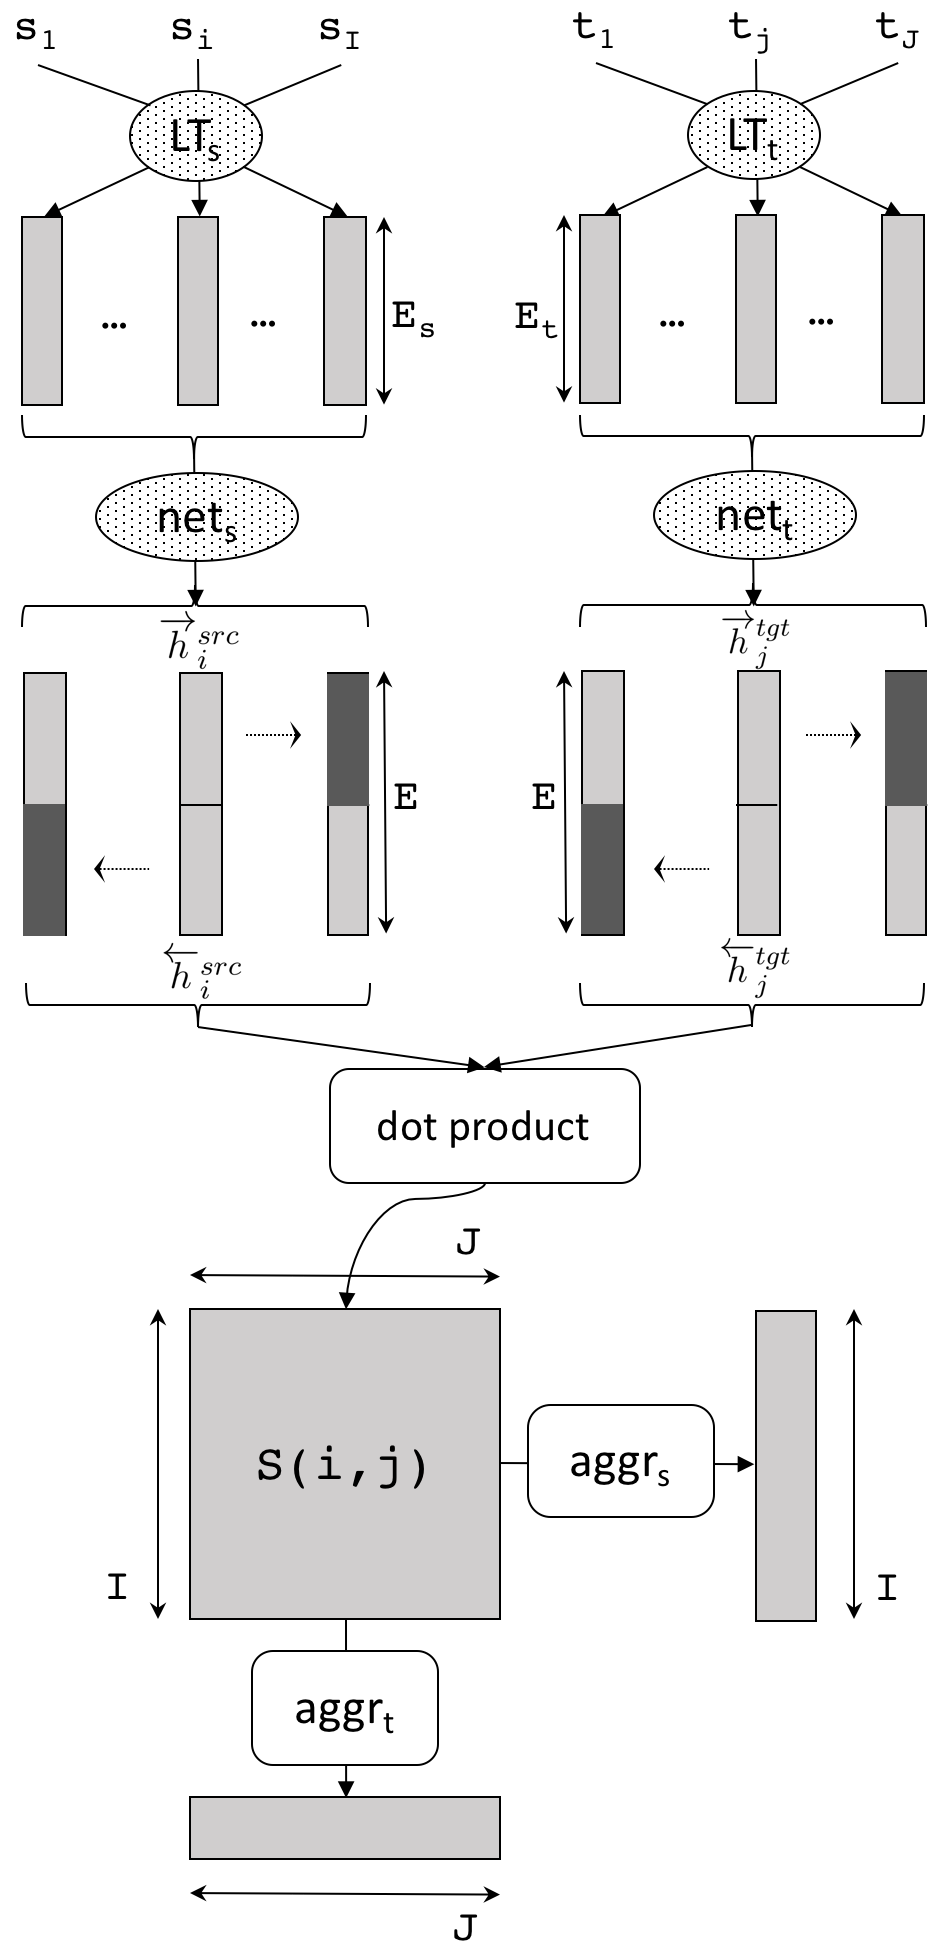
\includegraphics[width=1.0\linewidth]{network}
    \caption{Illustration of the model. The network is composed of source and target word embedding lookup tables ($LT_s$ and $LT_t$) and two identical subnetworks ($net_s$ and $net_t$) that compute in context representations of source ($s_i$) and target words ($t_j$).} 
    \label{network}
\end{figure}
%The similarity function outputs the level of semantic similarity between source and target sentences.

%Figure~\ref{net_lstm} illustrates the first component of our network. In order to optimise our model we follow the functions depicted in Figure~\ref{net_align}.

Similar to ~\cite{W16-2207} our model extracts context information from source and target sentences and then computes simple dot-products to estimate word alignments. The objective function is computed at the level of words. 
To enable unsupervised training, we use an aggregation operation that summarizes the alignment scores for a given target word. A soft-margin objective increases scores for true target words while decreasing scores for target words that are not present.
The aggregation function combines the scores of all source (or target) words for a particular target (or source) word and promotes source words which are likely to be aligned with a given target word according to the knowledge the model has learned so far.

Alignment scores $S(i,j)$ are given by the dot-product $S(i,j) = h_i^{src} \cdotp h_j^{tgt}$, while aggregation functions are defined as:

\begin{equation}
\begin{split}
    aggr_s(i,S) = \frac{1}{r} \ log \left( \displaystyle \sum_{j=1}^{J} e^{r * S(i,j)}\right) \\
    aggr_t(j,S) = \frac{1}{r} \ log \left( \displaystyle \sum_{i=1}^{I} e^{r * S(i,j)}\right)
\end{split}
\label{aggregation}
\end{equation}

%Hence, rather than sentence similarity our model optimises word alignments.
The loss function is defined as:

%\vspace{-8mm}
\begin{equation}
\begin{split}
\mathcal{L}(src,tgt) = & \\
    \sum_{i=1}^I log&\left(1+e^{aggr_{s}(i,S) * \mathcal{Y}_i^{src}}\right) +\\
 + \sum_{j=1}^J log&\left(1+e^{aggr_{t}(j,S) * \mathcal{Y}_j^{tgt}}\right)
\end{split}
\label{loss_wemb}
\end{equation}
\noindent where $\mathcal{Y}_i^{src}$ (or $\mathcal{Y}_j^{tgt}$) is a vector with reference labels containing $-1$ when the $i^{th}$ source word (or $j^{th}$ target word) is present in the translated target (or source) sentence, and $+1$ for divergent (unpaired) words. 

%\begin{figure}[h]
%\center
%    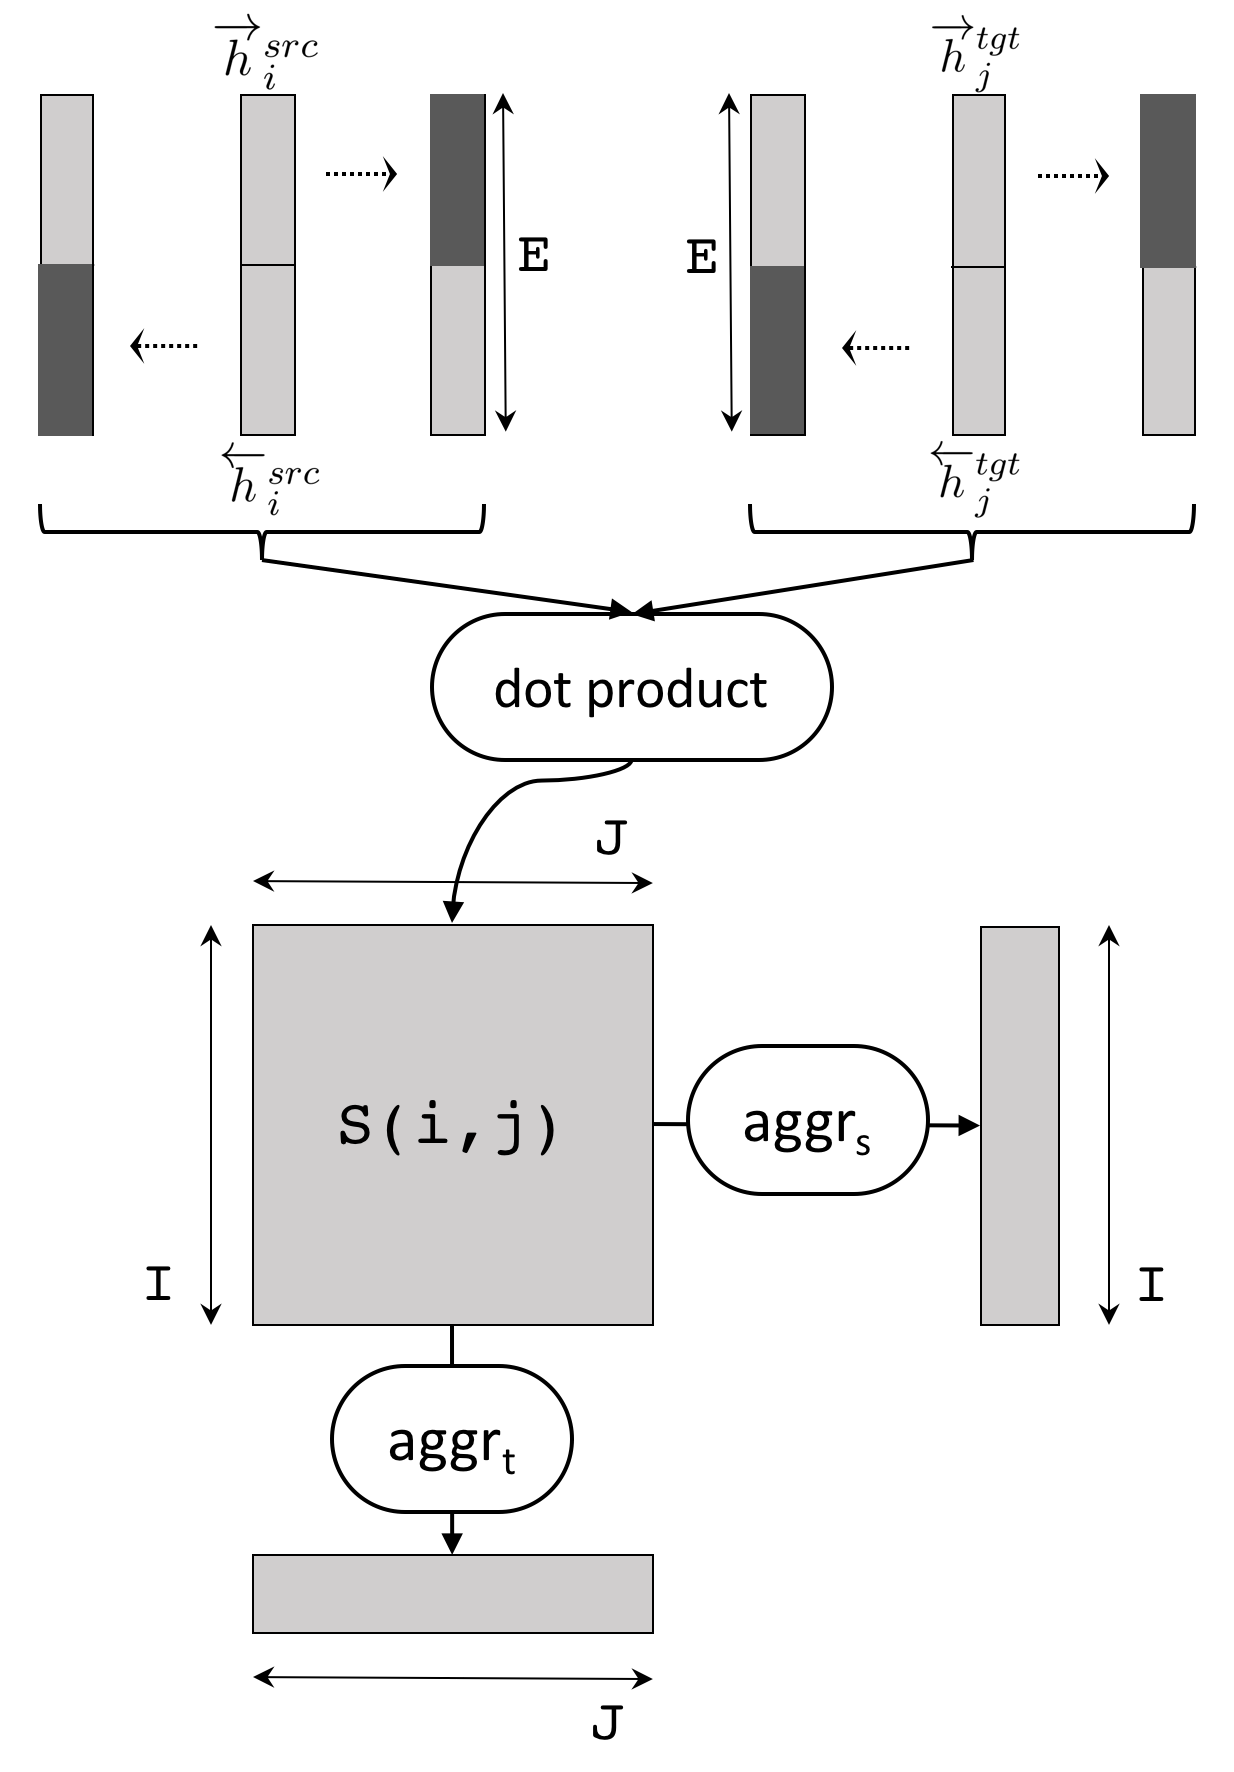
\includegraphics[width=0.9\linewidth]{net_align}
%    \caption{Illustration of the model.}
%    \label{net_align}
%\end{figure}

%\vspace{-8mm}

%For comparison purposes we also implemented the model introduced in \cite{W17-2509}. The network employs the same initial Bi-LSTM layers outlined in Figure~\ref{network} which encode source and target sentences into $h_{src}$ and $h_{tgt}$ vectors. The remaining of the network is illustrated by Figure~\ref{net_sentence}, where sentence pair matching information is captured by using their element-wise product and absolute element-wise difference. Sentence similarities are finally estimated by feeding the matching vectors into a fully connected layer.

%\begin{equation}
%\begin{split}
%h^{(1)} =  &\ \ h_{src} * h_{tgt} \\
%h^{(2)} =  &\ \ |h_{src} - h_{tgt}| \\
%h^{(3)} = &\ \ tanh(W[h^{(1)};h^{(2)}] + b^{(3)}) \\
%h_{sim} = &\ \ Wh^{(3)} + b^{sim}
%\end{split}
%\end{equation}

%This approach is different from our model since it uses a single end-to-end model to estimate the conditional probability distribution that two sentences are parallel. 

%\begin{figure}[h]
%\center
%    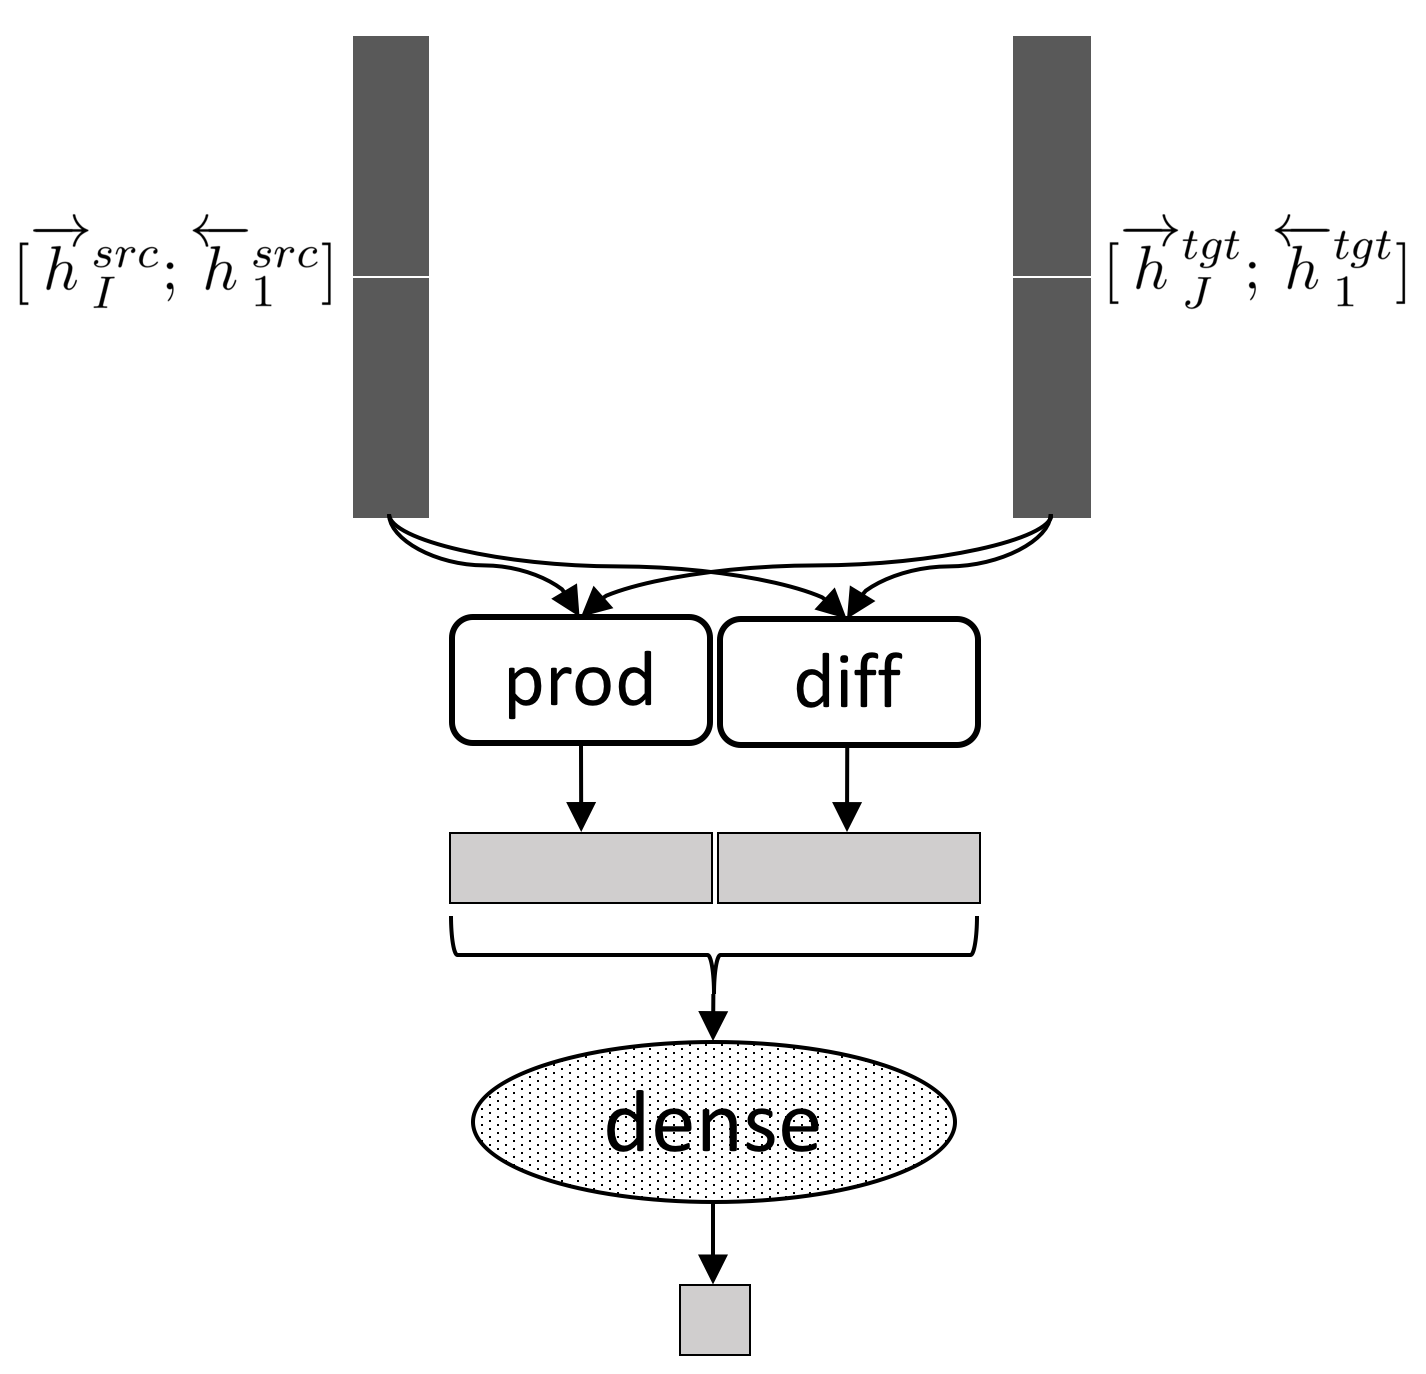
\includegraphics[width=0.8\linewidth]{net_sentence}
%    \caption{Illustration of the model presented in~\cite{W17-2509}. Sentence embeddings (vectors in dark grey) are computed by the same Bi-LSTM layers shown in Figure~\ref{network}.} %The network is composed of source and target word embedding lookup tables ($LT_s$ and $LT_t$) and two identical subnetworks ($net_s$ and $net_t$) that compute in context representations of source ($s_i$) and target words ($t_j$). The similarity function outputs the level of semantic similarity between source and target sentences.}
%    \label{net_sentence}
%\end{figure}

%For this second network the loss function is defined as: 
%\vspace{-5mm}
%\begin{equation}
%\mathcal{L}(src,tgt) = log(1+e^{h_{sim} * \mathcal{Y})}) % where $sign(src,tgt) =1
%\label{loss_semb}
%\end{equation}
%\noindent where $\mathcal{Y}$ is the reference label containing $-1$ when the given sentence pair is non-divergent (parallel) and $+1$ for divergent (unpair) examples. 

%Note that different from the network described in the original work, our implementation does not estimates a probability distribution but FINISH.

%For each source(target) word, we consider the aggregated matching score over the target(source) sentence:
%$$s_{aggr}(i,tgt) = Aggr_{j=1}^{J} s(i,j)$$
%$$s_{aggr}(src,j) = Aggr_{i=1}^{I} s(i,j)$$

%Where $Aggr$ is LSE aggregation operator used in~\cite{W16-2207}. Given the sign of each word noted $sign(w)$, that indicates whether the word $w$ is matched to the other side (by convention, $1$ indicates non-matching, $-1$ indicates matching), the loss function is defined as follows:


%In the second option, we directly optimize the score of similarity between two sentences by defining the loss function as follows:

%$$L(src,tgt) = log(1+e^{h_{src} . h_{tgt} * sign(src,tgt)})$$ where $sign(src,tgt) =1 $ if two sentences are not parallel and $sign(src,tgt) =-1 $ otherwise.

\subsection{Training with Negative Examples}
\label{training}

Training is performed by minimising Equation~\ref{loss_wemb}, for which examples with annotations for source $\mathcal{Y}_i^{src}$ and target $\mathcal{Y}_j^{tgt}$ words are needed.

As positive examples we use {\bf paired} sentences of a parallel corpus. All words of the pair of sentences are labelled as parallel, $\mathcal{Y}_i^{src}=-1$ and $\mathcal{Y}_j^{tgt}=-1$. 
As negative examples we use random {\bf unpaired} sentences. In this case, all words are labelled as divergent, $\mathcal{Y}_i^{src}=+1$ and $\mathcal{Y}_j^{tgt}=+1$. 
Since negative examples may be very easy to classify and we want our network to detect less obvious divergencies, we further create negative examples following the next two methods:

We {\bf replace} random sequences of words on either side of the sentence pair by a sequence of words with the same part-of-speeches. 
The rationale behind this method is to keep the new sentences as grammatical as possible. 
Otherwise the network can learn to detect non-grammatical sentences to predict divergence.
Words that are not replaced are considered parallel ($-1$) while those replaced are assigned the divergent label ($+1$). 
Words aligned to some replaced words are also assigned the divergent label ($+1$). For instance, given the original sentence pair:

\begin{table}[h]
\begin{tabular}{ll}
src: & { \small \texttt{What do you feel ?}} \\
tgt: & { \small \texttt{Que ressentez-vous ?}} \\
\end{tabular}
\end{table}

We may replace '\texttt{you feel}', with part-of-speech tags '\texttt{PRP VB}', by another sequence with same tags (i.e. '\texttt{we want}'):

\begin{table}[h]
\begin{tabular}{ll}
src: & { \small \texttt{What do {\bf we \ want} ?}} \\
$\mathcal{Y}^{src}$: & { \small \texttt{-1 \ \  -1 {\bf +1\ \ +1} \ \  -1}} \\
tgt: & { \small \texttt{Que {\bf voulez-vous} ?}} \\
$\mathcal{Y}^{tgt}$: & { \small \texttt{-1\ \ {\bf +1}\ \ \ \ \ \ \ -1}} \\
\end{tabular}
\end{table}

Divergent words are shown in bold. 
Note that the new sentences are not assured to be grammatical after replacing sequences with the same part-of-speech.
%Note that part-of-speeches and word alignments are needed to build this negative example. 
We use word alignments to identify as divergent the sequence '\texttt{ressentez-vous}' since it is aligned to the replaced sequence '\texttt{you feel}'.

Finally, motivated by sentence segmentation errors observed in many corpora, we also build negative examples by {\bf inserting} a second sentence at the beginning (or end) of the source (or target) sentence pair. 
Words in the original sentence pair are assigned the parallel label ($-1$) while the new words inserted are considered divergent ($+1$).
Given the original sentence pair previously shown, we may want to build the next negative example by inserting the sentence '\texttt{Not .}' at the end of the original source sentence:

\begin{table}[h]
\begin{tabular}{ll}
src: & { \small \texttt{What do you want ? {\bf Not \ .}}} \\
$\mathcal{Y}^{src}$: & { \small \texttt{-1 \ \  -1 -1 \ -1  \ \ -1 {\bf +1\ \ \  +1}}} \\
tgt: & { \small \texttt{Que ressentez-vous ?}} \\
$\mathcal{Y}^{tgt}$: & { \small \texttt{-1\ \ -1\ \ \ \ \ \ \ \ \ \ \ \ \ -1}} \\
\end{tabular}
\end{table}

In order to avoid that negative examples are easily predicted just by looking at the difference in length of training sentences we constraint all negative examples to have a difference in length not exceeding $2.0$. Very short sentences, up to $4$ words, are accepted if the length ratio does not exceeds $3.0$.

%The network outlined in Figure~\ref{net_sentence} uses a single label for each sentence pair. 
%Hence, positive examples are labelled $\mathcal{Y}=-1$ while any of the previously described negative examples are labelled $\mathcal{Y}=+1$.

\subsection{Fixing Translation Divergencies}
\label{correction}

We observed in our training corpus that many divergent sentences follow a common pattern, consisting of containing some extra leading/trailing words. See the first and second examples of table~\ref{tab:examples}. 
Accordingly, we implemented an algorithm that discards sequences of leading/trailing words making use of alignment scores $S(i,j)$. 
Hence considering as parallel $s_[^]$ and $t_\langle^\rangle$. To find the optimal source ($[, ]$) and target ($\langle, \rangle$) indexes that enclose the corrected segment within the original sentence, we implement:
%\vspace{-4mm}
\begin{equation*}
\begin{split}
%\underset{[, ], \{, \}}{\arg\max}&\{\mathcal{P}([,],\{,\}) - \mathcal{Q}([,],\{,\})\} \\
\underset{[, ], \langle, \rangle}{\arg\max}& \Big \{      \underset{[ \le i \le ]}{\sum} \underset{\langle \le j \le \rangle}{\max} \{ S(i,j) \}  \Big \} % -   \underset{[ > i, i > ]}{\sum} \underset{\langle > j, j > \rangle}{\max} \{ s(i,j) \}   \Big \}
\end{split}
\end{equation*}
%\noindent where $\mathcal{P}$ and $\mathcal{Q}$ are defined:
%\vspace{-4mm}
%\begin{equation*}
%\begin{split}
%\mathcal{P}&([,],\{,\}) = \underset{[ \le i \le ]}{\sum} \underset{\{ \le j \le \}}{\max} \{ s(i,j) \} \\%+ \underset{\{ \le j \le \}}{\sum} \underset{[ \le i \le ]}{\max} \{ s(i,j) \}  \} \\
%\mathcal{Q}&([,],\{,\}) = \underset{[ > i, i > ]}{\sum} \underset{\{ > j, j > \}}{\max} \{ s(i,j) \} %+ \underset{\{ > j < \}}{\sum} \underset{[ > i < ]}{\max} \{ s(i,j) \}  \} \\
%\end{split}
%\end{equation*}

The $\mathcal{N}$-best sequences following the previous function ($s_[^]$, $t_\langle^\rangle$) are considered as valid corrections, but only the highest ranked according to their similarity score is used as replacement for the original $(s_1^I, t_1^J)$. % if it has a higher similarity score: $sim(s_[^], t_\{^\}) > sim(s_1^I, t_1^J)$. 
Short sentences are not considered. This is, $] - [ > \tau$ and $\langle - \rangle > \tau$. 

Figure~\ref{matrix} (left) shows an example of an alignment matrix $s(i,j)$ for a given sentence pair. A possible correction is: \texttt{What do you feel ? $\Leftrightarrow$ Que ressentez-vous ?}. Hence, with indexes $[=1$, $]=5$, $\langle=1$ and $\rangle=3$.


%\begin{figure*}
%\centering
%\begin{multicols}{2}
%    \includegraphics[width=1.1\linewidth]{learn}    
%    \includegraphics[width=1.1\linewidth]{summer}    
%    \includegraphics[width=1.1\linewidth]{swim} 
%    \includegraphics[width=1.4\linewidth]{awesome}
%\end{multicols}
%\begin{multicols}{3}
%    \includegraphics[width=\linewidth]{sandwich}
%    \includegraphics[width=\linewidth]{sandwich}
%    \includegraphics[width=\linewidth]{peu}
%\end{multicols}
%\caption{Examples of neural alignment output by the matrix $S_{i,j}$ in Figure~\ref{network}. Only positive scores, indicating alignment between words $s_i$ and $t_j$, are printed. Different levels of grey are used to highlight the alignment.}
%\end{figure*}

\section{Experiments}
\label{experiments}

In this section we report on the experiments conducted to evaluate the proposed network. We begin with details of the corpora employed.

\subsection{Corpora}
\label{corpora}

Different corpora are used in this work to evaluate our similarity classifier.

We filter out divergencies found in the English-French OpenSubtitles corpus~\cite{LisonTiedemann2016}, which consists of a collection of movie and TV subtitles, aligned at the sentence level after a number of automatic preprocessing steps. 
The corpus presents many potential divergencies as outlined in Table~\ref{tab:examples}. 
To evaluate performance we used the En-Fr Microsoft Spoken Language Translation task, created from actual conversations over Skype~\cite{mslt-corpus-iwslt-2016-release}. 
%We also tested on a second domain, using the publicly available newstest-2013 En-Fr test set, corresponding to news stories selected from online sources~\cite{WMT:2013}.
In order to better assess the quality of our classifier when facing different types of word divergencies we collected from the original corpus and annotated at the word level $500$ sentences containing:
200 paired sentences;
100 unpaired sentences;
100 sentences with replace examples; and
100 sentences with insert examples as detailed in Section~\ref{training}.

We also use the Paracrawl corpus, which consists of a very noisy $1$ billion word (English token count) German-English corpus crawled from the web as part of the Paracrawl project\footnote{http://paracrawl.eu/}.
Performance is evaluated on the publicly available newstest-2017 En-De test set, corresponding to news stories selected from online sources~\cite{W17-4717}.

%To evaluate the ability of our sentence embeddings to identify parallel sentences in comparable corpora we followed the data conditions made available for the BUCC shared task~\cite{ZWEIGENBAUM18.12}. 
%For training we used the French-English European Parliament corpus from WMT15\footnote{http://www.statmt.org/wmt15/translation-task.html}.
%For testing we used the test set made available by the task organisers, consisting of about $300,000$ monolingual sentences per language, French and English, that contains near $10,000$ parallel sentences.
%Test data come from Wikipedia\footnote{http://ftp.acc.umu.se/mirror/wikimedia.org/dumps} and News Commentary\footnote{http://www.casmacat.eu/corpus/news-commentary.html}.

\subsection{Training}

All data used in this paper is preprocessed with an in-house toolkit that performs minimal tokenisation, basically splitting-off punctuation.

\subsubsection{Neural Similarity Classifier}
\label{divergence}

After tokenisation, each out-of-vocabulary word is mapped to a special UNK token.
Our similarity classifier is described in Section~\ref{sec:similarity}. 
Word embeddings ($LT_s$ and $LT_t$) are initialised using \texttt{fastText}\footnote{https://github.com/facebookresearch/fastText}, further aligned by means of \texttt{MUSE}\footnote{https://github.com/facebookresearch/MUSE} following the unsupervised method detailed in~\cite{lample2018word}. 
Size of embeddings is $E_s=E_t=256$ cells. 
Both Bi-LSTM use 256-dimensional hidden representations ($E=512$). 
Optimization of the parameters is done using the stochastic gradient descent method along with gradient clipping (rescaling gradients whose norm exceeds a threshold) to avoid the exploding gradients problem~\cite{Pascanu:2013:DTR:3042817.3043083}. 
For each epoch we randomly select $1$ million sentence pairs that we place in batches of $32$ examples.  
Negative examples are created following the strategies detailed in~\ref{training}.% ({\bf P}aired, {\bf U}unpaired, {\bf R}eplace and {\bf I}nsert).
We run $10$ epochs and start decaying at each epoch by $0.8$ when score on validation set increases. 

Two networks are evaluated. 
The first is the work presented in this paper, it optimises the loss shown by equation~\ref{loss_wemb}, and uses Equation~\ref{cosine} to compute similarity scores (\texttt{wemb}).
The second implements the work in~\cite{W17-2509}, it optimises the loss shown by Equation~\ref{loss_semb} which in an end-to-end fashion predicts wether two sentences are parallel (\texttt{semb}).
To fix translation divergencies we used $\mathcal{N}=20$ and $\tau=3$.

\subsubsection{Neural MT}
\label{translation}

In addition to the basic tokenisation we perform Byte-Pair Encoding~\cite{Sennrich2016} with $30,000$ merge operations learned from both English and French data.

We build our NMT systems based on the open-source project \texttt{OpenNMT}\footnote{http://opennmt.net}. We use a bidirectional RNN encoder with $4$ LSTM layers with each containing $1,000$ cells. Word embeddings have a size of $300$ cells. We set the dropout probability to $0.3$. Batch size is set to $64$. The maximum length of both source and target sentences is set to $80$. % and we limit the vocabulary size to $50K$ words for both source and target languages.
The default optimiser is SGD with the starting learning rate of $1.0$. We start to decay the learning rate from epoch $10$ or when we detect increasing perplexity as compared to the previous epoch on a validation set. We stop training after $20$ epochs.


\section{Results}
\label{sec:results}

We evaluate first the ability of our similarity classifier to predict different types of divergencies. 
We use the test set manually annotated for that purpose and train our model on the OpenSubtitles corpus.
The same number of paired examples (P) is used than for any other class (U, R or I). %This is, in the case of the model trained using with all types of examples, the same number of examples of each class is used.

\begin{table}[h]
\small
\center
\begin{tabular}{crccccc}
\hline
\multicolumn{2}{l}{\bf Accuracy} & \multicolumn{5}{c}{Test examples} \\
 &  & \texttt{P} & \texttt{U} & \texttt{R} & \texttt{I} & \texttt{PURI} \\
 \hline
\parbox[t]{0mm}{\multirow{7}{*}{\rotatebox[origin=c]{90}{Train examples}}} &  \texttt{PU}     & \bf 0.996 & \bf 0.994 & 0.671 & 0.673 & 0.874 \\
 &  \texttt{PR}     & \bf 0.995 &      0.033 & \bf 0.951 &      0.689 & 0.746 \\
 &  \texttt{PI}       & \bf 0.998 &      0.071 &      0.697 & \bf 0.725 & 0.705 \\
 &  \texttt{PUR}  & \bf 0.994 & \bf 0.989 & \bf 0.919 &      0.710 & 0.932 \\
 &  \texttt{PUI}    & \bf 0.995 & \bf 0.996 &      0.662 & \bf 0.769 & 0.887 \\
 &  \texttt{PRI}    & \bf 0.991 &      0.161 & \bf 0.924 & \bf 0.719 & 0.768 \\
 &  \texttt{PURI} & \bf 0.995 & \bf 0.980 & \bf 0.916 & \bf 0.788 & \bf 0.942 \\
\hline
\end{tabular}
\caption{Word divergence accuracies for networks trained with different combinations of negative examples. P, U, R and I stand respectively for pair, unpair, replace and insert.}
\label{results_puri}
\end{table}

Table~\ref{results_puri} shows accuracies obtained by our model when trained over different combinations of negative examples on the task of predicting wether words are divergent. 
We consider divergent those words for which the similarity score predicted by our model, Equation~\ref{cosine}, is negative.

As it can be seen, non-divergent words in parallel sentences (column \texttt{P}) are easy to identify. 
%In all cases the accuracy reaches $100\%$. 
Divergent words in unpaired sentences (column \texttt{U}) are also easy to identify as far as the model has seen unpaired examples in training. 
The accuracy drops dramatically when the model is not used to see unpaired sentences (rows  \texttt{PR}, \texttt{PI} and \texttt{PRI}).

Regarding columns \texttt{R} and \texttt{I}, accuracies are lower since these sentences contain a mix of divergent and non-divergent words. 
Hence, word divergence is more difficult to predict. 
Again, models that were trained with the corresponding examples obtain the highest accuracies (outlined in bold letters).
Column \texttt{PURI} shows accuracy results over the entire test set. This is, mixing all type of examples. 
The best accuracy is obtained by the system trained on all type of negative examples. 

%The test set was annotated after looking at the entire train set and looking for these type of examples. 
%Existance and distribution of types of 

\begin{figure}[h]
\centering
    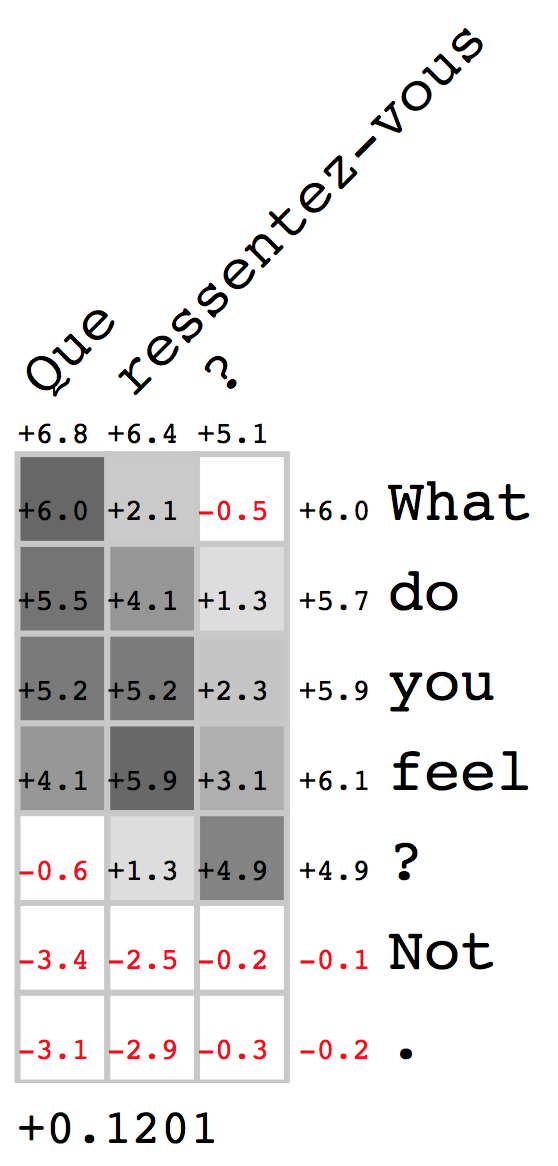
\includegraphics[width=0.4\linewidth]{feel}    
    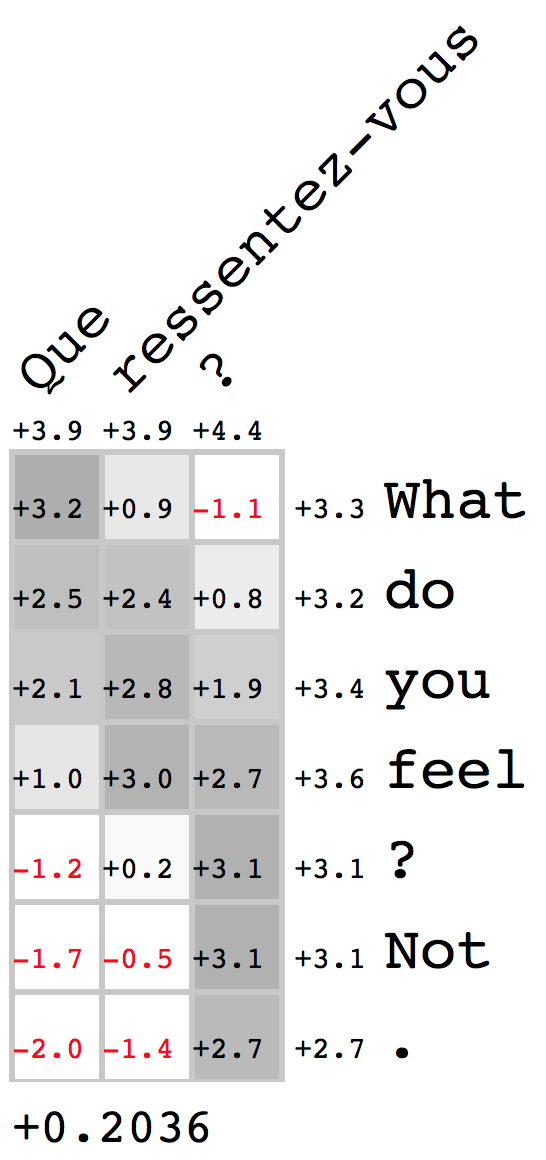
\includegraphics[width=0.4\linewidth]{feel_pu}    
\caption{Example of neural alignment matrices and divergence scores obtained with our model when trained over pair and unpair examples (right), and over all types of examples (left) as detailed in Section~\ref{training}. Aggregation scores of Equation~\ref{aggregation} are shown next to source and target words. Matrices contain word alignment scores. Sentence similarity scores computed by Equation~\ref{cosine} are shown below each matrix.}
\label{matrix}
\end{figure}

Figure~\ref{matrix} shows an example of word and sentence similarity predictions when our network is trained using all types of negative examples (left); and trained using only paired and unpaired sentences (right). 
As it can be seen, the network trained using examples where all words are either divergent or non-divergent (right), fails to correctly predict the class for words in sentences with mixed divergent/non-divergent words. In contrast, the model trained with all types of examples (left) correctly predicts the right class for each word. Furthermore, it correctly assigns a lower similarity score to the sentence pair, as both sentences do not convey the exact same meaning.

\subsection{Divergent Sentences Identification Task}

Next, we evaluate the ability of our neural similarity classifier to detect divergent sentence pairs. 
Since we lack of a gold standard test set to directly evaluate sentence similarity, 
we measure the accuracy of neural MT systems trained over the original corpus and after filtering divergent sentences. 
Notice that some divergent sentences may not be completely useless to train a neural MT system. 
Consider for instance the example of Figure~\ref{matrix}. 
Despite not conveying the exact same meaning it still contains useful information when training a neural MT engine. 
It is not the case of the example in the third row of Table~\ref{tab:examples}.

\begin{table}[h]
\small
\center
\begin{tabular}{lcc}
\hline
\bf $sim(h_{src},h_{tgt})$ & \bf Size (M) & \bf Test (BLEU)\\%& \bf NEWS \\
\hline
$(-\infty,+\infty)$   & 27.2 & 42.18 \\ %& 26.60  \\
$[0.000,+\infty)$   & 24.0 & 42.68 \\ %& 26.87  \\
$[0.003,+\infty)$   & 21.5 & 42.56 \\ %&  \\
$[0.076,+\infty)$   & 18.0 & \bf 43.19 \\ %& 26.38 \\
$[0.100,+\infty)$   & 15.5 & \\%&  \\
\hline
\end{tabular}
\caption{BLEU scores obtained by a neural MT network when trained over the OpenSubtitles corpus filtered using different similarity thresholds.}
\label{results_wemb}
\end{table}

Table~\ref{results_wemb} shows BLEU~\cite{P02-1040} scores of the same neural MT network when trained over different samples of the OpenSubtitles corpus.
Samples result from filtering sentences of the original corpus using different similarity thresholds.
As it can be seen, the best performing training sample is obtained when using sentence pairs with similarity score in the range $[0.076, +\infty)$. 
This is, training with the most similar $18$ million sentences of the original data set.

%Table~\ref{results_nmt} shows BLEU scores for the same neural MT system trained with different samples of the OpenSubtitles and Paracrawl corpus.
For each of the corpora, OpenSubtitles and Paracrawl, Table~\ref{results_nmt} shows BLEU scores of the neural MT system trained over the entire data set (\texttt{All}), and over the $18$ (and $15$) million sentences with highest similarity score as predicted by \texttt{semb} and \texttt{wemb} classifiers. REPHRASE

\begin{table}[h]
\small
\center
\begin{tabular}{lcc}
\hline
\bf Data & \bf Size (M) & \bf Test (BLEU) \\ %MSLT & \bf NEWS \\
\hline
\multicolumn{3}{c}{\scriptsize{OpenSubtitles English-French}} \\
\texttt{All}                    & 27.2 & 42.18 \\%& 26.60 \\ 
\texttt{semb}               & 18.0 & \\%&  \\
\texttt{wemb}              & 18.0 & 43.19 \\%& 26.38 \\
\hline
\multicolumn{3}{c}{\scriptsize{Paracrawl English-German}} \\
\texttt{All}                    & 100 & 12.56 \\ 
\texttt{base}                & 22.0 & 19.27 \\ 
\texttt{semb}               & 15.0 &  \\
\texttt{wemb}              & 15.0 &   \\
\hline
\end{tabular}
\caption{.}
\label{results_nmt}
\end{table}

%clean.min1.max99.maxw40.fert6-5-3.data.tok.en.lid.filtered
In the case of the Paracrawl corpus, we applied first a \texttt{base} filtering that reduced the amount of sentences to $22$ millions. 
It consists of limiting the sentence size to $100$ words. 
We also limit the length ratio between source/target sentences to $6$, and we employed an in-house language Id classifier that helped us to detect sentence pairs not being English-German. 

As it can be seen FINISH

\subsection{Parallel Sentences Identification Task}

\begin{table}[h]
\small
\center
\begin{tabular}{lrccccc}
\hline
\bf Model & $N=1$ & $10$ & $50$ & $100$ & $500$ & $1,000$ \\
\hline
\texttt{MUSE}           & & & & & & \\
\texttt{semb}            & & & & & & \\
\texttt{wemb}           & ssaling & & & & & \\
\hline
\end{tabular}
\caption{Number of parallel sentences found on the $N$-best cosine similarity filter (FAISS) according to the sentence embeddings produced by different networks.}
\label{results_embeddings}
\end{table}

The Cartesian product is costly for semb a filtering preprocess is necessary. Not for our model since we use faiss.

\begin{table}[h]
\small
\center
\begin{tabular}{lcccc}
\hline
\bf Model  & $\lambda$ & Precision & Recall & F-measure \\
\hline
\texttt{MUSE}             & & & & \\
\texttt{wemb}             & & & & \\
\texttt{semb}              & & & & \\
\hline
\end{tabular}
\caption{Precission, Recall and F-measure for the three evaluated models on the BUCC task.}
\label{results_similarity}
\end{table}

\section{Conclusions}
\label{conclusions}

We presented an unsupervised method based on deep neural networks for detecting translation divergencies in parallel sentence pairs. Our model also predicts misaligned words that can then be filtered out allowing for reusing some divergent sentences.
We evaluated our model on a neural machine translation task showing that it outperforms a baseline system trained on the entire (unfiltered) data set. The method can be used on any parallel corpus without any manual annotation.

\section{Further Work}
\label{further}

We plan to further evaluate divergence classification under larger data size conditions and different noise levels and on additional language pairs. 
%In this work we used a (noisy) parallel corpora to learn a divergence model. We also would like to evaluate the impact of using using less noisy (already filtered) data to learn the model. 
We also plan to study the use of a neural network to predict divergent words, as a replacement for the algorithm detailed in Section~\ref{correction}.

%\section*{Acknowledgements}
%We are grateful to Jo\"el Legrand for his fruitful comments when building the neural divergence classifier.

\bibliography{biblio}
\bibliographystyle{acl_natbib_nourl}

\end{document}
